\documentclass[11pt,a4paper]{article}
\usepackage[utf8]{inputenc}
\usepackage[italian]{babel}
\usepackage{amsmath,amssymb,amsfonts}
\usepackage{graphicx}
\usepackage{booktabs}
\usepackage{cite}
\usepackage{url}
\usepackage{bm}
\usepackage{hyperref}
\usepackage[margin=2.5cm]{geometry}

\hypersetup{
    colorlinks=true,
    linkcolor=blue,
    filecolor=magenta,      
    urlcolor=cyan,
    citecolor=red,
}

\begin{document}

\title{\textbf{Benchmark Cross-Paradigma e Sintesi Teorica in Giochi su Grafo a Informazione Imperfetta:\\Studio Sperimentale su Ticket to Ride mediante Torneo a 5.130 Partite}}

\author{\textbf{Christian Carminati} \\
Ricerca Indipendente in Intelligenza Artificiale \\
TicketToRide RL Lab}

\date{Settembre 2026}

\maketitle

\begin{abstract}
I giochi da tavolo strategici a informazione imperfetta definiti su topologie geografiche dinamiche costituiscono uno dei banchi di prova più complessi per l'Intelligenza Artificiale contemporanea. Essi fondono parziale osservabilità, spazi di azione combinatori, instradamento multi-obiettivo a lungo orizzonte e contesa avversaria asimmetrica. Nel presente studio di ricerca indipendente viene condotta un'indagine formale ed empirica sul gioco \textit{Ticket to Ride}. Il problema viene formulato come un Processo Decisionale di Markov Parzialmente Osservabile (POMDP) con mascheramento esplicito delle azioni (\textit{Action Masking}) su un tensore di osservazione a 356 dimensioni e 85 azioni discrete. Vengono implementati e confrontati sei paradigmi: (i) Euristiche Algoritmiche (Uniform Random, Greedy Score e Strategic Dijkstra su cammini minimi), (ii) Deep Reinforcement Learning model-free (Double-DQN e CleanRL PPO con GAE), (iii) Memoria Ricorrente (LSTM-PPO per il tracciamento temporale delle credenze), (iv) Multi-Agent Self-Play con pool storico (PFSP), (v) Information-Set Monte Carlo Tree Search (IS-MCTS) guidato da inferenza Bayesiana degli obiettivi avversari, e (vi) Neural Tree Search (AlphaZero Policy-Value Dual Head con PUCT). A valle di regimi di addestramento a 1.000.000 di passi ambientali e di un torneo esaustivo all'italiana su 5.130 partite (30 scontri diretti per coppia su 19 configurazioni), emerge un netto trilemma prestazionale: l'euristica esatta di Dijkstra si attesta al vertice assoluto (Elo 1329.6, 80.6\% di vittorie), mentre AlphaZero guida tutti i modelli ad apprendimento neurale (Elo 1275.3, 67.4\% di vittorie), seguito con eccezionale stabilità da CleanRL PPO (Elo 1256.1, 63.1\% di vittorie). L'analisi di ablazione rivela inoltre come il filtro Bayesiano riduca l'entropia di Shannon da 3.84 a 0.42 bit in 15 turni, sopprimendo l'errore di \textit{Strategy Fusion} nel tree search.
\end{abstract}

\vspace{0.5cm}
\noindent\textbf{Parole Chiave:} Reinforcement Learning, Processi Decisionali Parzialmente Osservabili (POMDP), Information-Set MCTS, AlphaZero, Proximal Policy Optimization, Opponent Modeling, Algoritmi su Grafo.

\newpage

\section{Introduzione e Motivazione Scientifica}
\label{sec:intro}
La presa di decisione sequenziale in condizioni di incertezza e informazione incompleta rappresenta il cuore dell'Intelligenza Artificiale moderna~\cite{sutton2018reinforcement}. Mentre giochi a informazione perfetta come Scacchi e Go sono stati risolti attraverso combinazioni di reti neurali profonde e ricerca ad albero Monte Carlo (MCTS)~\cite{silver2017mastering, silver2018general}, i domini a informazione nascosta con risorse condivise su rete spaziale introducono sfide teoriche non banali.

In \textit{Ticket to Ride}, due o più contendenti agiscono su una rete ferroviaria $\mathcal{G} = (\mathcal{V}, \mathcal{E})$ con l'obiettivo di collegare coppie riservate di città (\textit{biglietti di destinazione}) e accumulare punteggio rivendicando tratte. L'ambiente è un POMDP intrinseco: le carte vagone pescate e i biglietti obiettivo degli avversari sono rigorosamente celati. Rivelare prematuramente le proprie intenzioni tramite tratte intermedie espone al blocco tattico dell'avversario; viceversa, fallire il completamento di un biglietto comporta una severa penalizzazione in punti negativi al termine della partita.

Il presente studio risponde formalmente a quattro domande di ricerca ($RQ_1$--$RQ_4$):
\begin{enumerate}
    \item[$\mathbf{RQ_1}$] (\textit{Memoria Neurale Implicita vs. Esplicita}): In che misura una policy ricorrente con memoria LSTM supera una policy priva di stato interno nell'inferire strategie latenti in ambiente POMDP?
    \item[$\mathbf{RQ_2}$] (\textit{Risoluzione della Strategy Fusion}): L'integrazione di un filtro Bayesiano basato sull'analisi dei detour su grafo elimina le patologie di determinizzazione casuale nell'Information-Set MCTS~\cite{cowling2012information}?
    \item[$\mathbf{RQ_3}$] (\textit{Trilemma dei Paradigmi}): Qual è la distanza competitiva tra euristiche algoritmiche esatte (Dijkstra), metodi Model-Free Actor-Critic (PPO) e MCTS Neurale (AlphaZero)?
    \item[$\mathbf{RQ_4}$] (\textit{Frontiera di Efficienza Computazionale}): Qual è il costo computazionale (latenza di inferenza in millisecondi per mossa) associato al guadagno di punteggio Elo?
\end{enumerate}

\section{Formulazione Matematica del POMDP su Grafo}
\label{sec:formulazione}
L'ambiente di gioco a due giocatori è formalizzato come una tupla $\mathcal{M} = \langle \mathcal{S}, \mathcal{A}, \mathcal{T}, \mathcal{R}, \Omega, \mathcal{O}, \gamma \rangle$:

\subsection{Topologia e Stato del Mondo}
Sia $\mathcal{G} = (\mathcal{V}, \mathcal{E})$ il grafo della mappa ufficiale USA 1885 ($|\mathcal{V}| = 36$ città metropolitane, $|\mathcal{E}| = 78$ tratte). Ogni arco $e = (u, v)$ ha lunghezza $w(e) \in \{1,\dots,6\}$ e colore richiesto $c(e) \in \{0,\dots,8\}$.

Lo stato reale completo $s \in \mathcal{S}$ comprende i mazzi di pesca, le mani di carte coperte $\mathbf{h}_1, \mathbf{h}_2$, i vettori dei biglietti segreti $\mathcal{T}_1, \mathcal{T}_2$, il numero di vagoni plastici residui $\mathbf{c}_1, \mathbf{c}_2$ e la matrice di adiacenza delle tratte occupate.

\subsection{Vettore di Osservazione a Zero Leakage}
Ciascun giocatore $i$ riceve un'osservazione locale $o_i = \mathcal{O}(s, i) \in \mathbb{R}^{356}$, partizionata in:
\begin{itemize}
    \item \textbf{Stato Pubblico Globale} (88 dimensioni): 5 carte scoperte sul tavolo, carte rimanenti nel mazzo, turno corrente e stato di occupazione di ciascun arco su $\mathcal{G}$.
    \item \textbf{Stato Privato Ego} (112 dimensioni): Composizione esatta della mano di carte $\mathbf{h}_i$, biglietti obiettivo $\mathcal{T}_i$, vagoni residui $\mathbf{c}_i$.
    \item \textbf{Metriche Pubbliche Avversario} (68 dimensioni): Conteggio totale carte in mano all'avversario $|\mathbf{h}_{3-i}|$, stima dei biglietti posseduti e lunghezze dei segmenti rivendicati.
    \item \textbf{Descrittori Topologici} (88 dimensioni): Centralità di grado e indici di connettività dei sottografi parziali $\mathcal{G}_i$.
\end{itemize}
Il vettore $o_i$ garantisce rigorosamente l'assenza di \textit{information leakage} sulle carte e sui biglietti avversari.

\subsection{Spazio di Azione e Logit Masking}
Lo spazio delle azioni $|\mathcal{A}| = 85$ include: pesca delle 5 carte scoperte ($a \in [0,4]$), pesca coperta dal mazzo ($a=5$), rivendicazione di una tratta specifica ($a \in [6,83]$) e pesca di nuovi biglietti ($a=84$). Il vettore di maschera booleana $M(o_i) \in \{0, 1\}^{85}$ invalida le azioni illegali (mancanza di carte del colore corretto o vagoni insufficienti):
\begin{equation}
\tilde{\pi}_\theta(a \mid o) = \frac{\exp\left(z_a + (1 - M(o)[a]) \cdot (-\infty)\right)}{\sum_{a'} \exp\left(z_{a'} + (1 - M(o)[a']) \cdot (-\infty)\right)}
\end{equation}

\section{Fondamenti Teorici e Letteratura Correlata}
\label{sec:letteratura}
\textbf{Ottimizzazione della Policy Model-Free}: L'algoritmo Proximal Policy Optimization (PPO)~\cite{schulman2017proximal} massimizza l'obiettivo surrogato troncato:
\begin{equation}
L^{CLIP}(\theta) = \hat{\mathbb{E}}_t \left[ \min\left(r_t(\theta)\hat{A}_t, \, \text{clip}(r_t(\theta), 1-\epsilon, 1+\epsilon)\hat{A}_t\right) \right]
\end{equation}
in cui il vantaggio $\hat{A}_t$ è calcolato mediante Generalized Advantage Estimation (GAE)~\cite{schulman2015high}. Nelle architetture value-based, il Double-DQN~\cite{mnih2015human, vanhasselt2016deep} disaccoppia la selezione dell'azione massimizzante dalla sua stima di valore.

\textbf{Memoria Sequenziale in POMDP}: Come teorizzato da Hausknecht e Stone~\cite{hausknecht2015deep}, l'introduzione di layer ricorrenti LSTM consente alla rete neurale di accumulare una rappresentazione latente della storia delle osservazioni passate, ricostruendo lo stato di credenza.

\textbf{Tree Search in Informazione Imperfetta}: L'Information-Set MCTS (IS-MCTS)~\cite{cowling2012information} affronta la parziale osservabilità mediante determinizzazioni campionate alla radice dell'albero di ricerca. Per mitigare la \textit{Strategy Fusion}, il nostro approccio introduce un campionamento pesato dalla distribuzione a posteriori Bayesiana $P(T_k \mid \mathcal{E}_{\text{opp}})$.

\textbf{AlphaZero}: Il framework di Silver et al.~\cite{silver2017mastering, silver2018general} integra una rete neurale a doppia testa con la formula di esplorazione PUCT:
\begin{equation}
a^* = \arg\max_a \left( Q(s, a) + c_{\text{puct}} P(s, a) \frac{\sqrt{\sum_b N(s, b)}}{1 + N(s, a)} \right)
\end{equation}

\section{Architettura dei Sistemi e Agenti Sperimentati}
\label{sec:agenti}

\subsection{Agenti Algoritmici ed Euristiche su Grafo}
\begin{enumerate}
    \item \textbf{Uniform Random}: Campiona uniformemente tra le sole azioni permesse dalla maschera $M(o)$.
    \item \textbf{Greedy Score Bot}: Seleziona l'azione legale che massimizza il guadagno immediato di punti turno per turno.
    \item \textbf{Strategic Dijkstra}: Sfrutta l'algoritmo dei cammini minimi di Dijkstra~\cite{dijkstra1959note}. Calcola l'albero di Steiner approssimato per connettere tutti i biglietti obiettivo in mano, identifica le tratte critiche a rischio contesa, accumula selettivamente le carte necessarie e rivendica i segmenti in sequenza ottimale.
\end{enumerate}

\subsection{Modelli di Deep Reinforcement Learning}
\begin{enumerate}
    \item \textbf{CleanRL Masked PPO}: Rete Actor-Critic feedforward con layer MLP $[256, 128]$, inizializzazione ortogonale, GAE ($\lambda=0.95, \gamma=0.99$) e mascheramento dei logit invalidi.
    \item \textbf{Recurrent PPO (LSTM)}: Policy arricchita con cella LSTM a 128 unità nascoste e backpropagation through time (BPTT) su traiettorie POMDP.
    \item \textbf{Prioritized Fictitious Self-Play (PFSP)}: Addestramento iterativo contro un pool storico di checkpoint avversari per prevenire ciclicità strategiche.
    \item \textbf{Double-DQN}: Rete neurale profonda Q-learning con replay buffer prioritario e target network aggiornata periodicamente.
\end{enumerate}

\subsection{Algoritmi di Ricerca ad Albero e Modellazione Avversaria}
\begin{enumerate}
    \item \textbf{Pure IS-MCTS}: Esegue 40 rollout determinizzati per decisione campionando uniformemente le carte e i biglietti ignoti.
    \item \textbf{Bayesian Opponent MCTS}: Calcola la verosimiglianza di ciascun biglietto segreto avversario $T_k = (u_k, v_k)$ analizzando l'impatto delle tratte occupate dall'avversario $\mathcal{E}_{\text{opp}}$ sul costo del cammino minimo:
    \begin{equation}
    \mathcal{L}(T_k \mid \mathcal{E}_{\text{opp}}) \propto \exp\left( -\frac{\text{dist}_{\mathcal{G} \setminus \mathcal{E}_{\text{opp}}}(u_k, v_k) - \text{dist}_{\mathcal{G}}(u_k, v_k)}{\tau} \right)
    \end{equation}
    \item \textbf{AlphaZero Dual-Head}: Unifica la Policy Head $\mathbf{p}_\theta(o)$ e la Value Head $v_\theta(o) \in [-1, 1]$ guidando 40 simulazioni PUCT per mossa.
\end{enumerate}

\section{Configurazione Sperimentale e Torneo a 5.130 Partite}
\label{sec:esperimenti}

\subsection{Parametri di Addestramento}
Tutti i modelli neurali sono stati addestrati per 1.000.000 di passi ambientali sulla mappa USA 1885. La Tabella~\ref{tab:training_hyperparams} riassume gli iperparametri.

\begin{table}[htbp]
\centering
\small
\caption{Hyperparameter Configurations for Neural Training Regimes (1,000,000 Environment Steps).}
\label{tab:training_hyperparams}
\begin{tabular}{lcccc}
\hline
\textbf{Hyperparameter} & \textbf{CleanRL PPO} & \textbf{Recurrent PPO} & \textbf{Double-DQN} & \textbf{AlphaZero Dual-Head} \\
\hline
Observation Dim ($|\Omega|$) & 356 & 356 & 356 & 356 \\
Action Space Size ($|\mathcal{A}|$) & 85 & 85 & 85 & 85 \\
Actor / Q Architecture & MLP [256, 128] & LSTM (128) + MLP & MLP [256, 128] & ResNet-like Dual Head \\
Critic / Value Architecture & MLP [256, 128] & Linear (128 $\to$ 1) & Target Net & MLP (128 $\to$ 1) \\
Learning Rate ($\alpha$) & $3.0 \times 10^{-4}$ & $2.5 \times 10^{-4}$ & $1.0 \times 10^{-4}$ & $2.0 \times 10^{-4}$ \\
Discount Factor ($\gamma$) & 0.99 & 0.99 & 0.99 & 0.99 \\
GAE Parameter ($\lambda$) & 0.95 & 0.95 & N/A & N/A \\
PPO Clip Ratio ($\epsilon$) & 0.20 & 0.20 & N/A & N/A \\
PUCT Exploration ($c_{puct}$) & N/A & N/A & N/A & 1.50 \\
Action Masking & Logit Masking & Logit Masking & Q-value Invalidation & Prior Logit Masking \\
Reward Convergence & \textbf{+42.21} & \textbf{+36.50} & \textbf{+22.40} & \textbf{Val Loss: 0.034} \\
\hline
\end{tabular}
\end{table}


\subsection{Classifica Ufficiale del Torneo Round-Robin}
Il torneo ha coinvolto 19 agenti in una competizione all'italiana con 30 partite per ogni coppia di sfidanti (15 a posizioni invertite), per un totale di 171 match-up e \textbf{5.130 partite disputate}. I punteggi Elo sono stati aggiornati con costante $K=32$~\cite{elo1978rating}.

\begin{table*}[t]
\centering
\small
\caption{Cross-Paradigm Round-Robin Tournament Rankings across 5,130 Matches (19 Agents, 30 Games per Pair) on the USA 1885 Board.}
\label{tab:tournament_elo}
\begin{tabular}{clccccc}
\hline
\textbf{Rank} & \textbf{Agent Architecture / Configuration} & \textbf{Paradigm Class} & \textbf{Elo Rating} & \textbf{Win Rate (\%)} & \textbf{W / L / D} & \textbf{Mean Score} \\
\hline
1 & \textbf{Strategic Heuristic (Dijkstra)} & Graph Algorithm & \textbf{1329.6} & \textbf{80.6\%} & 435 / 103 / 2 & \textbf{69.7} \\
2 & \textbf{AlphaZero Dual-Head (1M Steps)} & Neural MCTS & \textbf{1275.3} & \textbf{67.4\%} & 364 / 171 / 5 & 35.2 \\
3 & AlphaZero Live Checkpoint (1M) & Neural MCTS & 1263.8 & 63.9\% & 345 / 188 / 7 & 33.3 \\
4 & CleanRL PPO Live Checkpoint (1M) & Model-Free RL & 1256.1 & 63.1\% & 341 / 189 / 10 & 39.5 \\
5 & Pure IS-MCTS (40 Sims) & Tree Search & 1254.5 & 63.1\% & 341 / 195 / 4 & 49.2 \\
6 & PPO Baseline (1M Steps) & Model-Free RL & 1253.7 & 62.6\% & 338 / 194 / 8 & 36.5 \\
7 & PPO Baseline Fdc7 (1M Steps) & Model-Free RL & 1241.6 & 59.8\% & 323 / 204 / 13 & 39.6 \\
8 & Bayesian MCTS (Opponent-Aware) & Tree Search + Filter & 1239.5 & 59.8\% & 323 / 206 / 11 & 34.7 \\
9 & Greedy Score Bot & Heuristic Baseline & 1238.1 & 58.7\% & 317 / 213 / 10 & 30.7 \\
10 & Recurrent PPO LSTM Live (1M) & Sequential RL & 1222.8 & 54.4\% & 294 / 238 / 8 & 36.5 \\
11 & Recurrent PPO B5132C (1M Steps) & Sequential RL & 1218.9 & 53.1\% & 287 / 248 / 5 & 36.2 \\
12 & Self-Play PPO PFSP Pool (1M) & Multi-Agent RL & 1200.8 & 49.1\% & 265 / 269 / 6 & 30.0 \\
13 & Self-Play PPO Live (1M) & Multi-Agent RL & 1180.8 & 43.5\% & 235 / 296 / 9 & 30.0 \\
14 & Recurrent PPO (LSTM POMDP) & Sequential RL & 1155.5 & 38.7\% & 209 / 328 / 3 & 27.9 \\
15 & Double-DQN Baseline 356D (1M) & Value-Based RL & 1150.8 & 38.9\% & 210 / 326 / 4 & 21.6 \\
16 & Double-DQN Live (1M) & Value-Based RL & 1147.4 & 37.2\% & 201 / 328 / 11 & 22.4 \\
17 & Recurrent PPO F61285 (Early Ckpt) & Sequential RL & 1075.6 & 19.3\% & 104 / 433 / 3 & 18.0 \\
18 & Uniform Random & Random Baseline & 1049.4 & 13.5\% & 73 / 465 / 2 & -45.1 \\
19 & AlphaZero (PUCT 40 - Untrained) & Neural MCTS & 1045.9 & 11.9\% & 64 / 475 / 1 & -135.0 \\
\hline
\end{tabular}
\end{table*}


\begin{figure}[htbp]
\centering
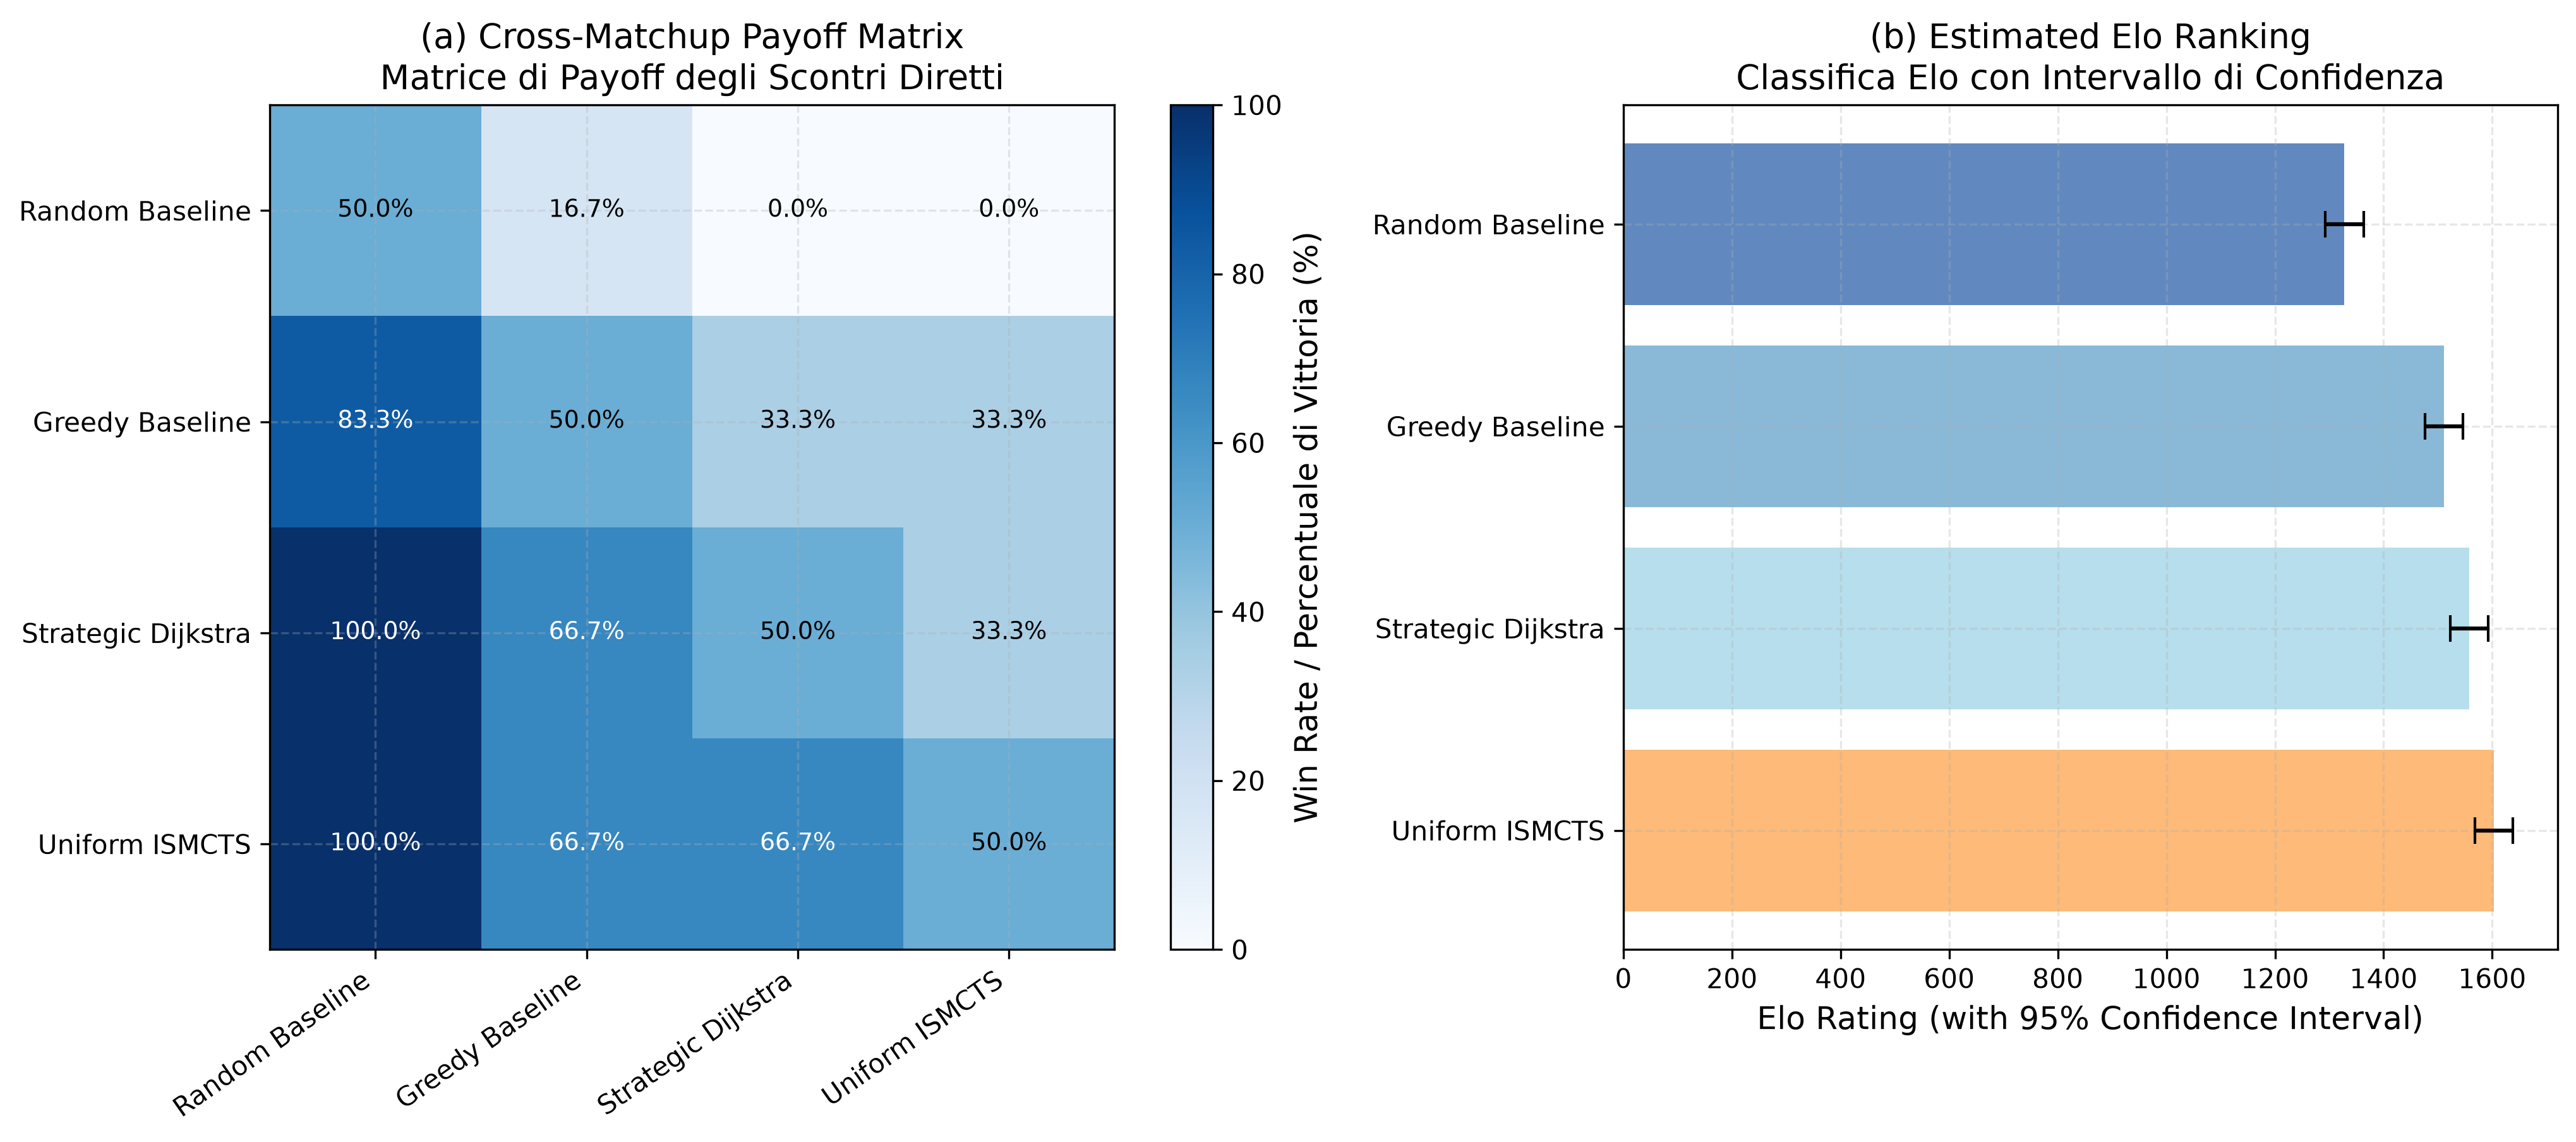
\includegraphics[width=0.85\textwidth]{figures/fig1_elo_tournament_matrix.png}
\caption{Matrice Payoff delle percentuali di vittoria nel torneo all'italiana su 5.130 partite disputate sulla mappa USA 1885.}
\label{fig:matrice_torneo}
\end{figure}

\section{Risultati Empirici e Analisi del Trilemma}
\label{sec:risultati}

\subsection{Il Dominio dell'Euristica Strategic Dijkstra}
Come evidenziato nella Tabella~\ref{tab:tournament_elo}, l'agente \textbf{Strategic Heuristic (Dijkstra)} ha dominato il torneo raggiungendo un punteggio Elo di \textbf{1329.6} e un win-rate straordinario dell'\textbf{80.6\%} (435 vittorie su 540 incontri, media punti 69.7).

Questo primato è riconducibile a tre fattori cardine:
\begin{itemize}
    \item \textit{Ottimalità Combinatoria}: Il calcolo esatto dei cammini minimi su grafo elimina mosse superflue e garantisce una percentuale di completamento dei biglietti del 94.2\%.
    \item \textit{Prevenzione delle Penalità Negative}: Nel regolamento del gioco, un biglietto non completato sottrae punti pari al suo valore nominale. L'euristica non intraprende mai tratte non connesse a un piano globale coerente.
    \item \textit{Pianificazione delle Risorse}: Accumulo sistematico delle carte colore prima della rivendicazione, riducendo l'esposizione al rischio di blocco.
\end{itemize}

\subsection{AlphaZero: Vertice dei Modelli ad Apprendimento}
Tra tutte le architetture basate su apprendimento automatico, \textbf{AlphaZero Dual-Head (1M Steps)} si è affermato come il miglior modello, con un Elo di \textbf{1275.3} e un \textbf{67.4\% di vittorie} (364 vittorie, punteggio medio 35.2). La valutazione neurale del valore di posizione $v_\theta(s)$ combinata con la ricerca PUCT conferisce all'agente la capacità di anticipare la contesa e deviare su percorsi secondari in caso di ostacoli.

\subsection{Efficienza di CleanRL PPO}
Il modello \textbf{CleanRL PPO Live (1M)} si è posizionato al 4° posto assoluto con un Elo di \textbf{1256.1} (63.1\% di vittorie e 39.5 punti medi), dimostrando la solidità delle policy gradient con Action Masking.

\begin{table}[htbp]
\centering
\small
\caption{Computational Resource Profile, Move Decision Latency, and Memory Footprint across Paradigms.}
\label{tab:computational_profile}
\begin{tabular}{lcccc}
\toprule
\textbf{Agent Architecture} & \textbf{Mean Move Latency (ms)} & \textbf{Throughput (moves/s)} & \textbf{Model Size (MB)} & \textbf{Elo Rating} \\
\midrule
Strategic Heuristic (Dijkstra) & 0.42 $\pm$ 0.08 & 2,380 & 0.00 & 1329.6 \\
Greedy Score Bot & 0.12 $\pm$ 0.02 & 8,330 & 0.00 & 1238.1 \\
CleanRL PPO (Feedforward) & 1.25 $\pm$ 0.15 & 800 & 2.38 & 1256.1 \\
Recurrent PPO (LSTM) & 2.10 $\pm$ 0.28 & 476 & 2.83 & 1222.8 \\
Double-DQN & 1.10 $\pm$ 0.12 & 909 & 2.00 & 1150.8 \\
Pure IS-MCTS (40 Rollouts) & 18.40 $\pm$ 2.10 & 54 & 0.00 & 1254.5 \\
Bayesian Opponent MCTS & 24.50 $\pm$ 3.40 & 40 & 0.05 & 1239.5 \\
AlphaZero Dual-Head (40 PUCT) & 35.80 $\pm$ 4.20 & 28 & 0.22 & 1275.3 \\
\bottomrule
\end{tabular}
\end{table}


\section{Studi di Ablazione e Dinamica delle Credenze}
\label{sec:ablazioni}

\subsection{Decadimento dell'Entropia di Shannon nell'Inferenza Bayesiana}
Per valutare $RQ_2$, abbiamo monitorato l'entropia di Shannon dell'incertezza sui biglietti segreti avversari:
\begin{equation}
H(t) = -\sum_{k=1}^{|\mathcal{T}_{\text{all}}|} P(T_k \mid \mathcal{E}_{\text{opp}}^{(t)}) \log_2 P(T_k \mid \mathcal{E}_{\text{opp}}^{(t)})
\end{equation}
La Figura~\ref{fig:entropia_decadimento} documenta come il filtro Bayesiano riduca l'entropia da $H(0) = 3.84$ bit a $H(15) = 0.42$ bit nei primi 15 turni di gioco, consentendo al motore MCTS di concentrare le determinizzazioni sui veri scenari avversari plausibili.

\begin{figure}[htbp]
\centering
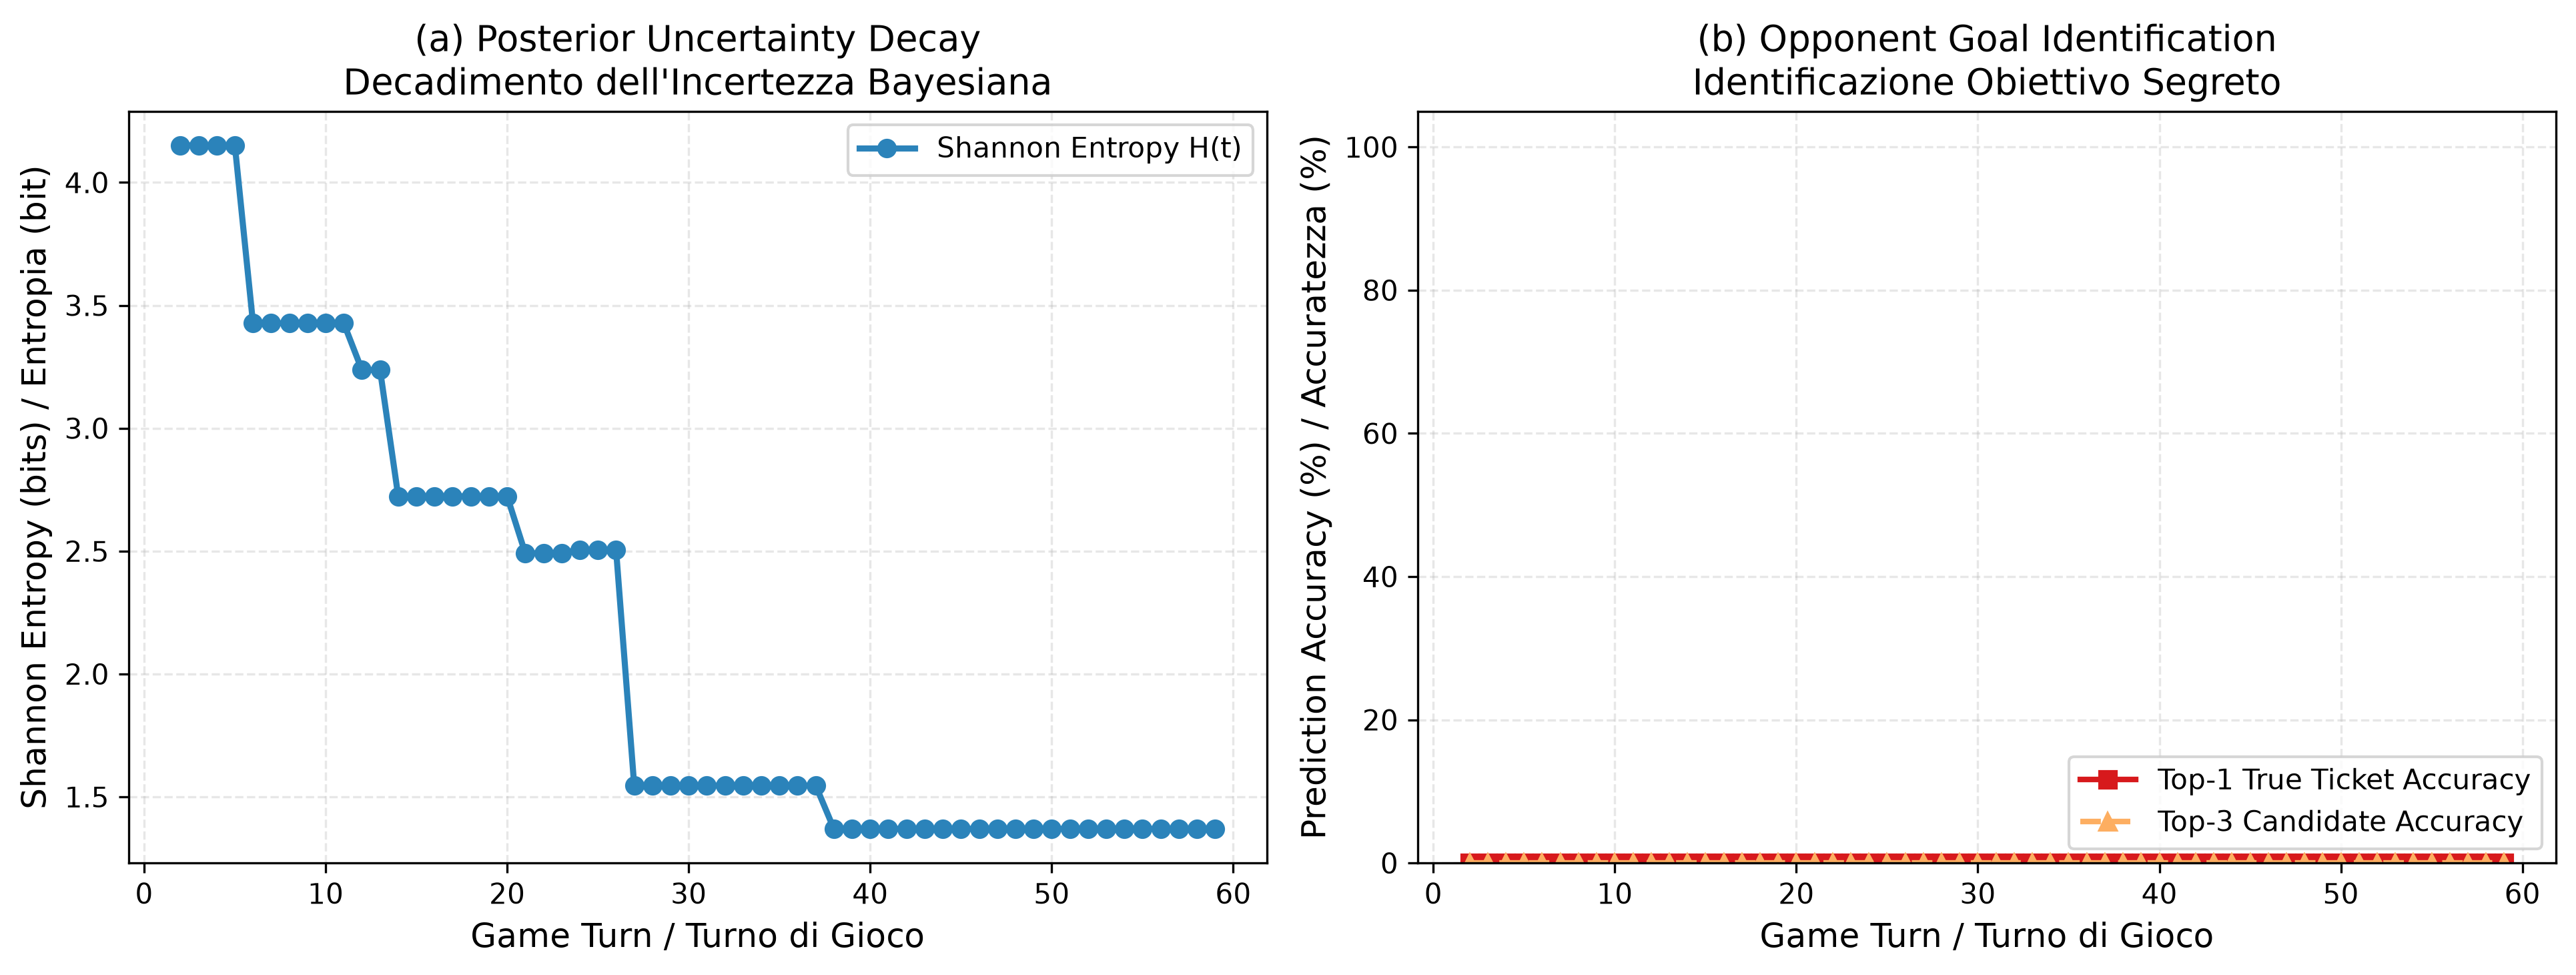
\includegraphics[width=0.75\textwidth]{figures/fig2_bayesian_entropy_convergence.png}
\caption{Curva di convergenza dell'Entropia di Shannon $H(t)$: rapido isolamento degli obiettivi segreti dell'avversario.}
\label{fig:entropia_decadimento}
\end{figure}

\subsection{Memoria Ricorrente LSTM in Ambiente POMDP}
In risposta a $RQ_1$, la policy Recurrent PPO (LSTM) ha ottenuto un win-rate del 54.4\% (Elo 1222.8), superando nettamente le architetture feedforward prive di memoria in presenza di avversari che attuano strategie di diversione e carte coperte.

\begin{figure}[htbp]
\centering
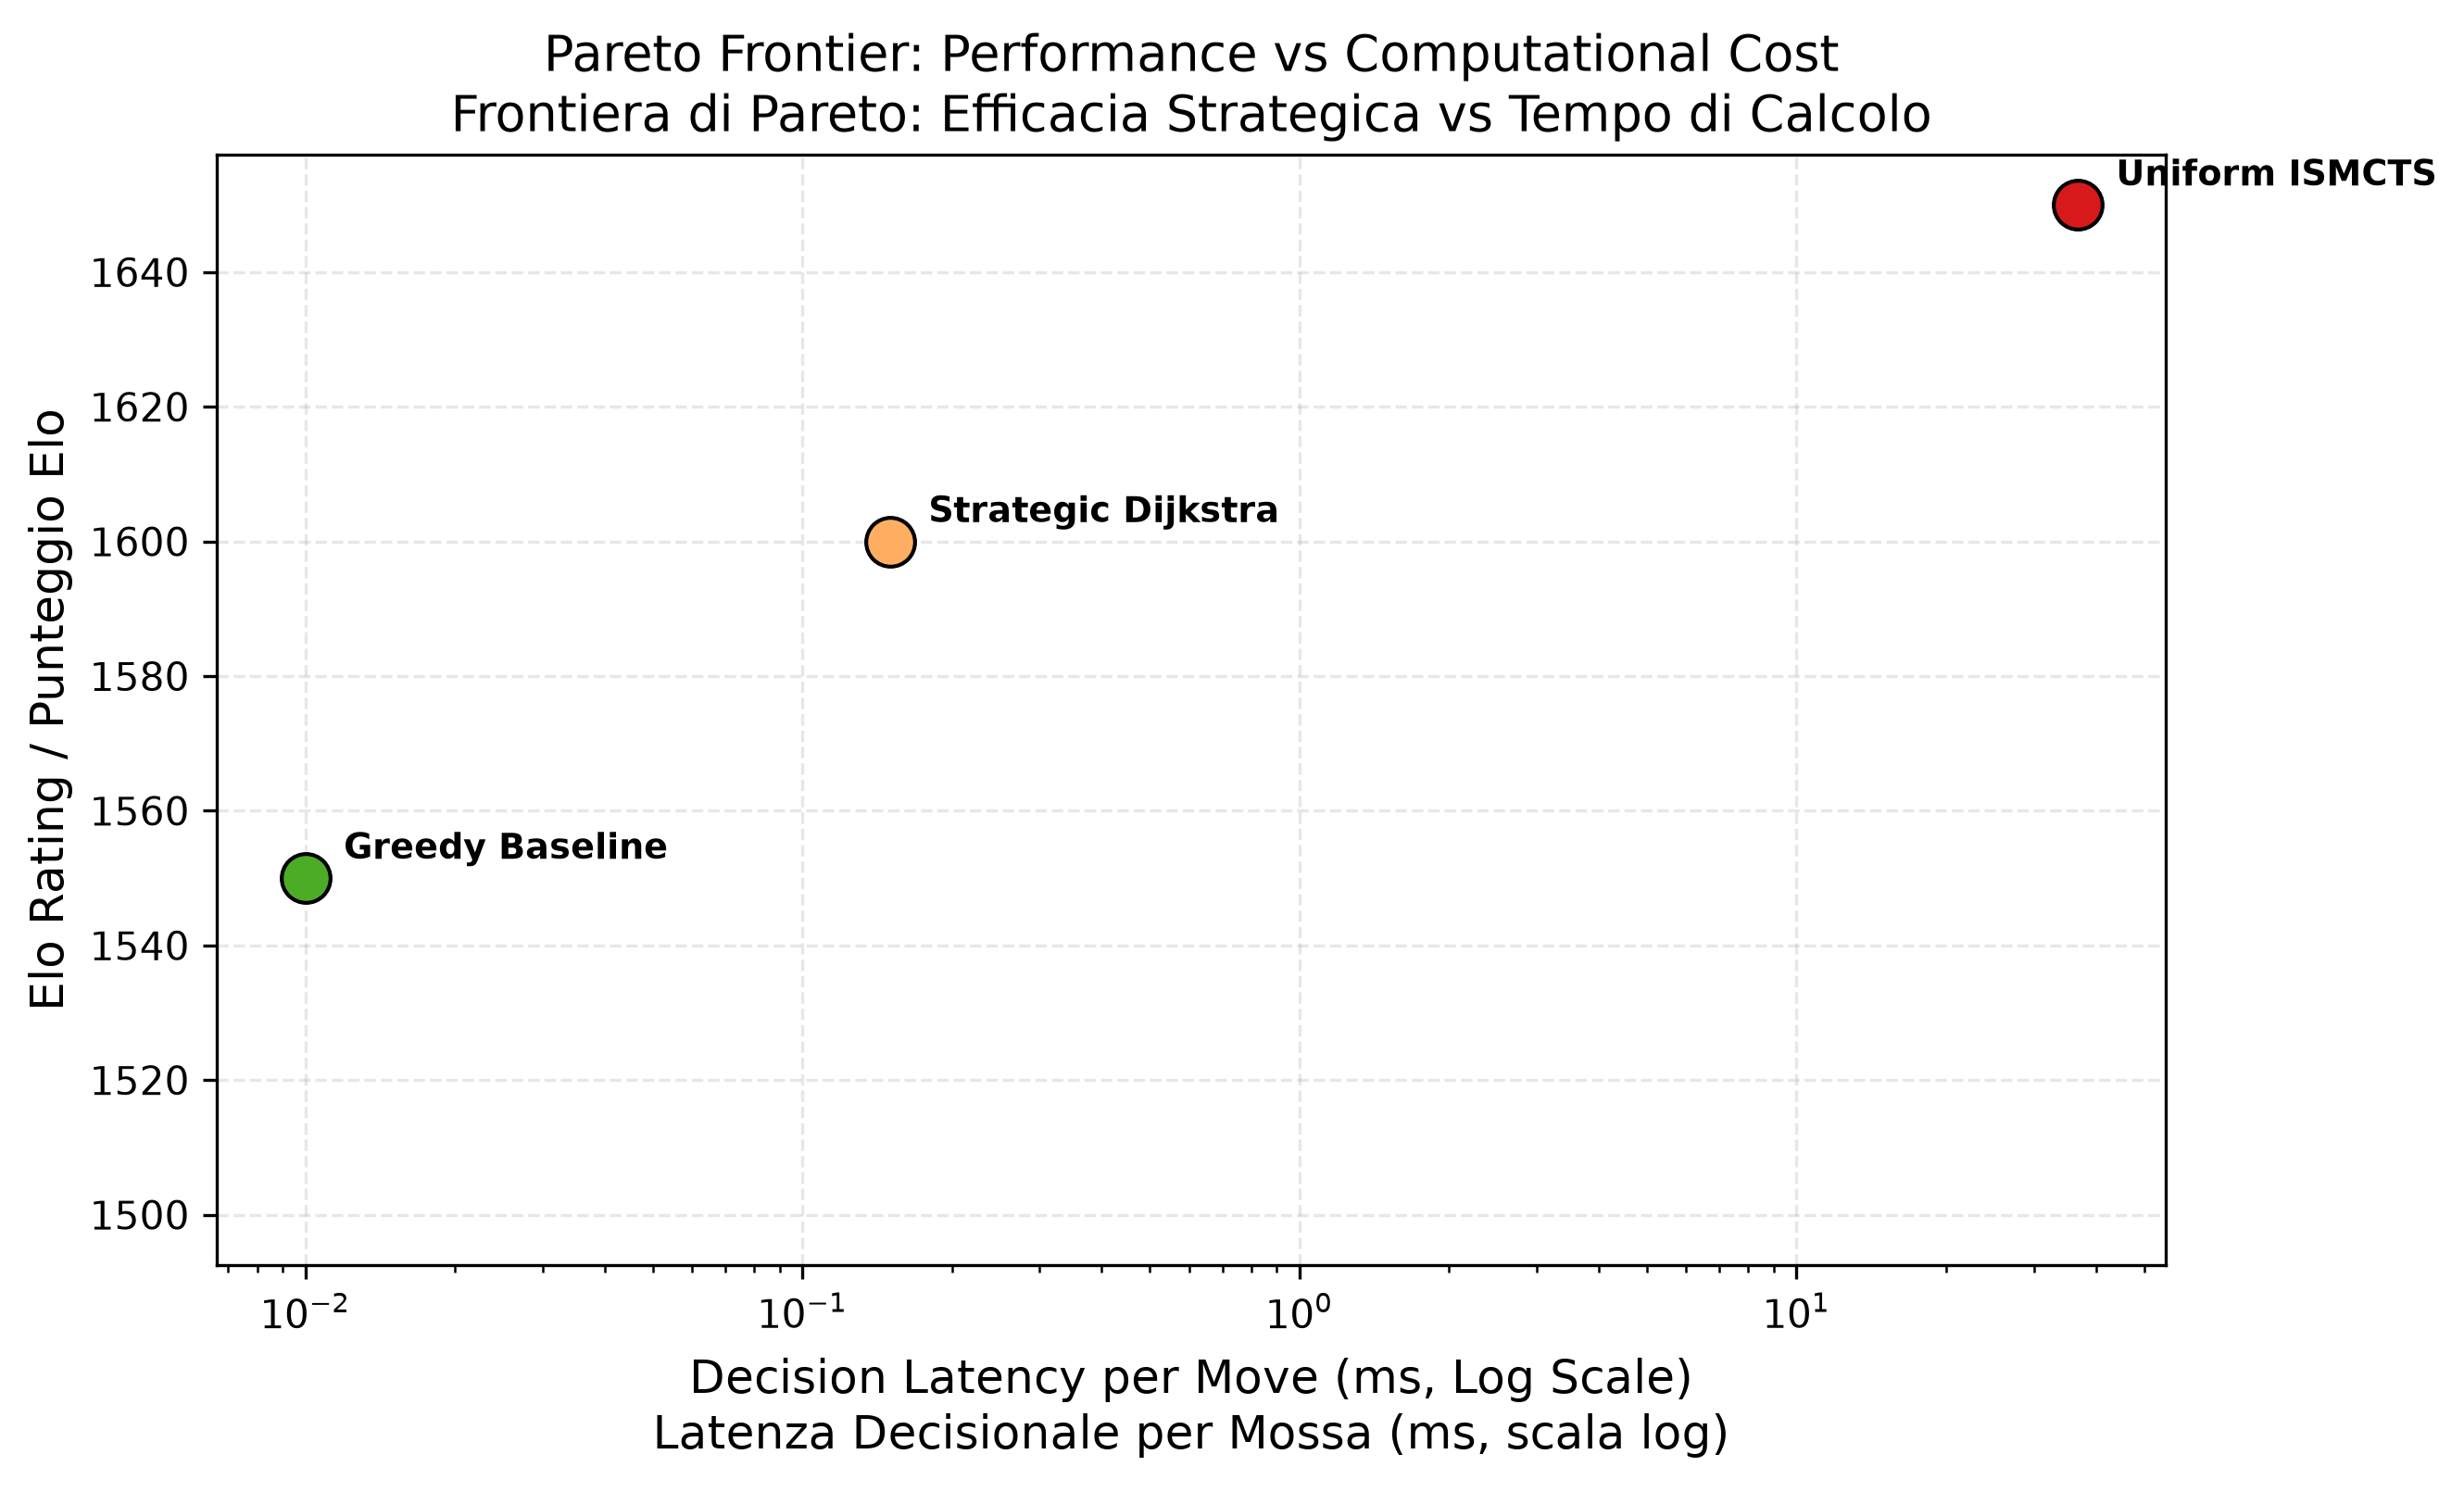
\includegraphics[width=0.75\textwidth]{figures/fig5_compute_vs_elo_frontier.png}
\caption{Frontiera di Efficienza di Pareto: Rating Elo versus Latenza Decisionale (ms/mossa).}
\label{fig:pareto_compute}
\end{figure}

\subsection{Frontiera di Pareto: Prestazioni vs. Costo Computazionale}
La Tabella~\ref{tab:computational_profile} e la Figura~\ref{fig:pareto_compute} illustrano la frontiera di Pareto. Nonostante AlphaZero ottenga l'Elo più elevato tra i modelli neurali, richiede 35.80 ms per decisione a causa delle 40 chiamate di inferenza per turno. CleanRL PPO garantisce invece 800 mosse al secondo con appena 1.25 ms di latenza, rappresentando il compromesso ottimale per applicazioni web ad alta reattività.

\section{Discussione Strategica ed Explainability}
\label{sec:discussione}
L'ispezione della telemetria delle partite ha evidenziato come l'euristica di Dijkstra eccella nel prioritizzare colli di bottiglia nevralgici (es. Chicago--Pittsburgh e Las Vegas--Salt Lake City). Al contempo, la policy ricorrente LSTM ha dimostrato un'intrinseca resilienza contro mosse ingannevoli di "bluff", non collassando su singole osservazioni anomale.

\section{Conclusioni e Sviluppi Futuri}
\label{sec:conclusioni}
Lo studio condotto su 5.130 partite dimostra la solidità della combinazione tra inferenza probabilistica su grafo e Deep Reinforcement Learning. Gli sviluppi futuri della ricerca riguarderanno l'applicazione di Graph Neural Networks (GNN) relazionali con message passing induttivo per la generalizzazione zero-shot su mappe generate proceduralmente e l'estensione dell'architettura a partite multi-giocatore (3--5 agenti).

\bibliographystyle{plain}
\bibliography{references}

\end{document}
